%!TeX root=../thesis.tex

\chapter{Analisis Permasalahan dan Solusi}

  % Pada bab ini akan dipaparkan analisis berdasarkan studi literatur pada bab sebelumnya terkait pembangunan sistem pencegahan intrusi berbasis GPU. Selain itu, akan dipaparkan juga solusi yang diajukan untuk mesin yang akan dibuat.

  \section{Analisis Permasalahan}
  
    % Sistem pencegah intrusi jaringan (NIPS) adalah sistem yang bertugas melakukan penyaringan paket yang dianggap berbahaya. NIPS bekerja dengan cara menangkap paket yang berjalan dalam jaringan untuk kemudian dianalisis. Hasil analisis kemudian ditindaklanjuti berdasarkan \emph{rule} yang telah didefinisikan. Paket dapat ditolak, dibatasi atau bahkan diblok.

    % Analisis paket dapat dilakukan dengan bermacam-macam metode asd

    Dampak dari pengecekan paket adalah adanya \emph{overhead} waktu respons. Lama \emph{overhead} tergantung dari waktu pencocokan pola. Pada sistem pencegah intrusi jaringan (NIPS), hal ini dapat membuat hasil analisis menjadi tidak akurat. Maka perlu adanya metode untuk mempercepat proses analisis. Sebagai perbandingan, \emph{bandwidth} jaringan US Naval Postgraduate School sudah mencapai 20 Gbps dengan traffic rata-rata sebesar 200 Mbps per hari. Sedangkan maksimum paket yang dapat dianalisis secara serial oleh Snort tidak lebih besar dari 300 Mbps \citep{albin2012}.

    Beberapa penelitian tentang teknik mempercepat NIDS dan NIPS telah dilakukan. Desain paling awal yaitu menggunakan desain konkuren dengan \emph{multithreading} pada CPU \citep{multi2004}. Desain ini mampu meningkatkan penggunaan utilitas \emph{thread} CPU secara drastis. Kemudian desain berbeda yang menggunakan GPU mulai diajukan oleh \citep{gnort2008}. Hasil yang didapat mampu mempercepat sistem hingga 5x dibandingkan CPU dengan harga yang sepadan \citep{smith2009}.

    % Pencocokan dapat dilakukan secara stateful, ataupun tidak. Pencocokan yang berbasis stateful akan lebih susah untuk dicek secara paralel.

    %Meski demikian, masih ada beberapa masalah terjadi dalam desain yang telah diajukan. Pencocokan paket masih menggunakan algoritma yang berbasis backtracking sehingga banyak operasi sinkronisasi yang menghambat laju pencocokan dengan multithread.  Selain itu, opsi pada rule seringkali tidak dapat dicocokkan dengan sekali asd

    Berdasarkan pengukuran yang dilakukan oleh \citep{kargus2012}, didapatkan bahwa sebagian besar beban analisa paket berada pada tahap pencarian string pada \emph{payload} paket. Pada tahapan ini, sebagian besar paket yang tidak terindikasi sebagai serangan akan diloloskan. Sehingga beban pencocokan pada tahap berikutnya, yaitu pencocokan \emph{option rule} akan berkurang drastis. Maka, fokus dari solusi yang akan diajukan yaitu implementasi desain yang akan mempercepat kinerja pencocokan string paket pada NIDS Snort.

  \section{Analisis Solusi}

    Eksperimen penggunaan GPGPU pada NIDS akan memodifikasi NIDPS Snort. Snort digunakan karena kode bersifat \emph{open-source} dan mudah untuk dikembangkan, sehingga pengembangan dan eksperimen tidak memerlukan banyak biaya dan dapat dieksplorasi secara mandiri. 

    Pengembangan akan menggunakan platform GPGPU CUDA. Platform CUDA merupakan platform GPGPU yang dibuat pada GPU NVIDIA. Platform CUDA digunakan karena saat ini platform CUDA lebih matang daripada OpenCL. Selain itu, dokumentasi dan contoh CUDA lebih banyak dan API yang lebih sederhana dan spesifik dibanding OpenCL.

    \subsection{Pemilihan Algoritma Pencocokan \emph{Signature}}

      Komponen utama yang akan dioptimasi yaitu pencocokan string. Diantara pencocokan pola yang digunakan pada Snort, versi Aho-Corasick memiliki runtime yang paling cepat menggunakan teknik multithreading pada CPU. Idealnya, modul yang ingin dikembangkan akan melampaui kinerja dari Snort yang menggunakan algoritma ini.
      
      Berdasarkan pengujian eksperimen yang dilakukan oleh \citep{lin2013}, implementasi langsung dari algoritma ini tidak memiliki keunggulan yang berarti pada GPU. Salah satu kendala dari algoritma AC (Aho-Corasick) adalah \emph{boundary matching problem}. Masalah ini bisa diatasi dengan menambahkan jangkauan pencarian sebesar pola terpanjang. Namun, efek dari trik ini adalah peningkatan kompleksitas yang cukup drastis dari $(O(n)$ menjadi $O(n + ms)$. 
      
      Solusi yang diajukan dalam \citep{lin2013} yaitu dengan menggunakan algoritma PFAC (\emph{Paralel Failureless Aho-Corasick}). PFAC adalah varian dari AC yang memulai pencocokan \emph{thread} pada tiap karakter dan tidak menggunakan \emph{failure transition}. Ada beberapa keuntungan dari algoritma ini:
    
      \begin{enumerate}

        \item 
        Tiap \emph{thread} hanya bertanggung jawab dengan string yang dimulai dengan karakter pada \emph{thread} tersebut. Ketika tidak ada pola yang cocok dengan huruf pada \emph{thread}, pencarian langsung berhenti pada \emph{thread}. Akibantnya, umur \emph{thread} juga lebih singkat tanpa adanya \emph{failure transition}

        \item
        Pencocokan pola dengan tabel transisi adalah aplikasi yang \emph{memory-bound}. Ketika pencocokan dilakukan, \emph{thread} yang bersebelahan akan mengakses karakter yang sebelumnya diakses oleh \emph{thread} lain. Berdasarkan skenario ini, akan lebih baik jika string disalin ke \emph{shared memory}.

        \item 
        Dalam mesin PFAC, tiap 32 \emph{thread} dalam \emph{warp} akan mengakses memori yang berurutan dari memori global. Dengan demikian, fitur \emph{memory coalescing} dapat dimanfaatkan.

        \item
        Memori yang lebih sedikit sebagai akibat tidak adanya \emph{failure transition}.

      \end{enumerate}

    % \subsection{Skema Pengiriman Paket ke GPU}

    %  Operasi yang cukup sering akan dilakukan dalam Snort NIPS adalah pengiriman paket dari stream 
    %  Salah satu komponen yang paling penting dalam GPGPU adalah penyalinan data antar host dan device. Pengiriman dari host ke device maupun sebaliknya memiliki \emph{latency} yang cukup besar. Dalam pengujian pada \citep{gnort2008}, didapatkan bahwa \emph{latency} dari transfer payload memiliki runtime lebih dari 80\% runtime total. Sehingga untuk menyembunyikan \emph{latency}, pengujian akan menggunakan batch processing.      
    % pengiriman akan dilakukan per batch. Ukuran batch yang digunakan akan diuji dalam ukuran 32MB, 64MB, 128MB, dan 256MB.

    \subsection{Pemilihan Struktur Penyimpanan \emph{Signature}}

      Implementasi dari mesin PFAC yang digunakan ada beberapa macam. Salah satu model yang dapat digunakan yaitu dengan bentuk seperti pohon dengan \emph{list of pointer} ke status anak. Namun, model yang dialokasi secara dinamis tidak cocok digunakan dalam GPU karena alokasi pada GPU memiliki latensi yang tinggi. Selain itu, lokasi memori dapat tidak koontigu dan tidak mendukung adanya \emph{spatial locality}.
      
      Opsi lainnya yaitu dengan tabel transisi dua dimensi. Untuk tiap status, akan dibuat daftar status transisi terhadap tiap karakter. Model ini lebih sederhana dan juga mendukung adanya \emph{spatial locality}. Tabel akan dibentuk di \emph{host memory}. Setelah semua pola didaftarkan, tabel akan disalin ke GPU hanya sebesar ukuran tabel yang terisi agar tidak boros memori.

      % Penyimpanan \emph{signature} mempengaruhi besar memori yang digunakan. Struktur yang digunakan akan menggunakan trie terkompresi. Struktur digunakan untuk memaksimalkan \emph{locality} sehingga mengurangi \emph{latency}. Selain itu, dengan menurunkan konsumsi memori, besar buffer yang dapat digunakan meningkat. Diharapkan, \emph{latency} dari pengiriman juga menurun.

      % Penggunaan texture memory diharapkan dapat membantu menurunkan latency dalam pembacaan tabel.

    \subsection{Pemilihan Teknik untuk Optimasi Implementasi pada GPU}

      Untuk mendukung operasi pencocokan, perlu ada teknik untuk menurunkan latensi pada GPU. Penyimpanan pola pada memori global adalah salah satu sumber latensi. Salah satu optimasi yang dapat digunakan yaitu menyimpan pola pada memori konstanta atau tekstur.

      Memori konstanta unggul ketika pola yang dicocokkan sedikit bercabang. Jika pola yang dicocokkan sedikit bercabang, maka \emph{cache} dapat dimanfaatkan dan latensi berkurang secara signifikan. Namun, pada ruleset Talos, tidak banyak rule yang sama sehingga juga akan banyak terjadi \emph{cache miss}. Akibatnya memori konstanta tidak lagi unggul. 
      
      Sementara itu, memori tesktur tetap dapat digunakan untuk mengurangi latensi pada simpul yang berdekatan. Berdasarkan \citep{lin2013}, penggunaan memori tekstur dapat meningkatkan kinerja hingga 12\%.

      Berikutnya adalah mengurangi latensi dari pembacaan masukan melalui global memori. Seperti yang telah disebutkan pada poin pertama, \emph{thread} yang bersebelahan akan sempat mengakses karakter yang sama. Sehingga tidak perlu melakukan akses terhadap memori global terus menerus. Masukan dapat disalin ke dalam \emph{shared memory} terlebih dahulu. Kemudian pencocokan dapat membaca langsung dari \emph{shared memory}.

  \section{Rancangan Solusi}

    Pembahasan mengenai rancangan solusi dibagi menjadi 3 bagian. Bagian pertama dibahas mengenai gambaran umum solusi. Bagian kedua dibahas mengenai kebutuhan perangkat lunak. Bagian ketiga dibahas arsitektur perangkat lunak. 

    \subsection{Gambaran Umum Solusi}

      Berdasarkan  analisis  yang  telah  dilakukan, terpilih beberapa metode yang akan digunakan dalam NIDS yang akan dibangun. Algoritma pencocokan yang akan digunakan adalah PFAC. Tabel transisi akan menggunakan tabel dua dimensi. Kemudian tabel ini akan diikat ke memori tekstur.

      Secara garis besar, terdapat 4 tahapan yang harus dilakukan dalam modul pencocokan pola yang akan dibangun, yaitu

      \begin{enumerate}

      \item
      Pembentukan tabel transisi \\
      Pembentukan tabel transisi akan dilakukan saat persiapan pencocokan. Pembentukan dilakukan pada \emph{host} kemudian baru akan ditransfer ke \emph{device}. Pembentukan tabel transisi dilakukan dengan mengumpulkan pola terlebih dahulu. Setelah pola terkumpul, lalu simpul akan disusun kembali agar simpul akhir berada di bagian paling awal tabel. 

      \item
      Persiapan tabel transisi dalam \emph{device memory} \\
      Setelah tabel transisi dibentuk, tabel akan dikirimkan ke \emph{device memory}. Penyimpanan pola akan diikat pada memori tekstur. Selain itu juga disiapkan tabel untuk menampung hasil pencocokan.

      \item
      Penelusuran automata \\
      Pencocokan dilakukan dengan penelusuran mesin PFAC yang sudah dibentuk. String masukan akan dimuat pada \emph{shared memory}. Tiap \emph{thread} akan memulai pencocokan pada satu karakter di string masukan. Penelusuran dilakukan hingga mencapai status akhir. Jika status akhir bukan merupakan status dummy, maka hasil pencocokan akan diset pada tabel yang berada di global memori.

      \item
      Penggabungan hasil pencocokan \\
      Hasil pencocokan berada di tabel pada global memori. Untuk menjumlahkan hasil pencocokan, beberapa teknik dapat dilakukan. Salah satu teknik yaitu \emph{interleaved addressing}. Kemudian dapat pula menggunakan optimasi seperti menjumlahkan ketika pertama kali memuat isi tabel. 

      \end{enumerate}

    \subsection{Kebutuhan Perangkat Lunak}

      Berdasarkan analisis yang dilakukan sebelumnya, NIDS yang akan dibangun setidaknya memiliki spesifikasi kebutuhan fungsional seperti yang dijabarkan dalam Tabel III.1.
      
      \begin {table}[h]
\begin{center}
\caption {Kebutuhan Fungsional}
\begin{tabular}{|p{.5cm}|l|}

\hline
\rowcolor{gray!10}
No & Kebutuhan Fungsional \\
\hline

1 & Mampu membaca paket dari berkas PCAP \\
\hline

2 & Mampu membuat struktur automata untuk pencocokan paket \\
\hline

3 & Mampu menjalankan pencocokan pada GPU \\
\hline

4 & Mampu menghasilkan \emph{alert} pada paket yang terindikasi berbahaya \\
\hline

\end{tabular}
\end{center}
\end{table}


      Berdasarkan Kebutuhan fungsional tersebut maka \emph{use case diagram} dari NIDS yang akan dibangun adalah seperti pada Gambar III.2 berikut

    \subsection{Arsitektur Perangkat Lunak}

      Arsitektur yang digunakan akan menggunakan arsitektur dasar Snort. Dalam mengimplementasikan modul pencocokan, Snort menyediakan antarmuka yang dapat dieksten dengan mudah. Sehingga dalam penggabungan modul tersebut, hanya perlu dibuat wrapper untuk memanggil modul yang telah diimplementasi secara terpisah.

      \begin{figure}[htb]
        \centering
        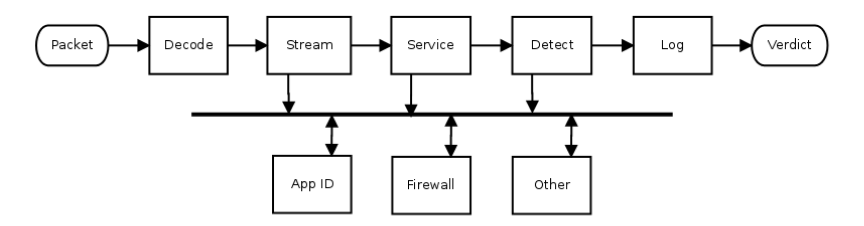
\includegraphics[width=0.8\textwidth]{resources/snort3.png}
        \caption[Arsitektur Snort versi 3]{Arsitektur Snort versi 3}
      \end{figure}

     % Berdasarkan analisis kebutuhan yang dijelaskan subbab sebelumnya, proses pengindeksan dan proses pencarian bisa dipisahkan karena dalam proses pencarian yang dibutuhkan hanyalah hasil indeks yang sudah jadi. Sehingga arsitektur solusi akan terbagi menjadi 2 buah sistem yaitu sistem untuk  pengindeksan dan sistem untuk pencarian.